\subsection{Explicación}
\begin{frame}
	\begin{block}{Enunciado}
	Dado un conjunto de ciudades y una matriz con las distancias entre todas ellas, un 			viajante debe recorrer todas las ciudades exactamente una vez, regresando al punto
	de partida, de forma tal que la distancia recorrida sea mínima.
	\end{block}
	\begin{exampleblock}{Solución}
	Permutación del conjunto de ciudades que indica el orden en que se deben recorrer
	\end{exampleblock}
\end{frame}

%%%%%%%%%%%%%%%%%%%%%%%%%%%%%%%%%%%%%%%%%%
\begin{frame}
	\begin{block}{Algoritmo}
	Nos centraremos en una serie de algoritmos aproximados de tipo greedy y evaluaremos
	su rendimiento en un conjunto de instancias.
	\end{block}
	\begin{block}{Greedy usados}
		\begin{itemize}
		\item Vecino más cercano
		\item Inserción de vértices
		\item Inserción de aristas
		\end{itemize}
	\end{block}
\end{frame}
%%%%%%%%%%%%%%%%%%%%%%%%%%%%%%%%%%%%%%%%%%5

\subsection{Vecino más cercano}
\begin{frame}
	\begin{block}{Desarrollo del algoritmo}
	Primero escogeremos una ciudad de inicio. Después calculamos las distancias de esa
	ciudad al resto y escogemos la más cercana. A partir de esa ciudad volvemos a calcular
	la ciudad más cercana y procedemos hasta pasar por todos los vértices.
	\end{block}

	\begin{alertblock}{Aviso}
	No debemos olvidar incluir el camino del último vértice al inicial, ya que forma parte
	del problema y hay que sumar también esa distancia.
	\end{alertblock}
\end{frame}

%%%%%%%%%%%%%%%%%%%%%%%%%%%%%%%%%
\subsubsection{Desarrollo visual}
\begin{frame}
	\begin{exampleblock}{Paso 1}
	\begin{figure}[htbH]
		\centering
		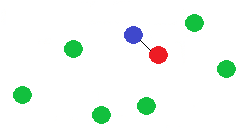
\includegraphics[width=0.65\textwidth]{./Imagenes/vecino1.png}
		\caption{Tercer vértice}
	\end{figure}
	\end{exampleblock}
\end{frame}

\begin{frame}
	\begin{exampleblock}{Paso 2}
	\begin{figure}[htbH]
		\centering
		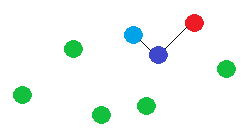
\includegraphics[width=0.65\textwidth]{./Imagenes/vecino2.png}
		\caption{Tercer vértice}
	\end{figure}
	\end{exampleblock}
\end{frame}

\begin{frame}
	\begin{exampleblock}{Paso 3}
	\begin{figure}[htbH]
		\centering
		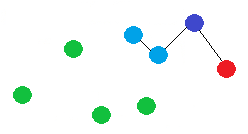
\includegraphics[width=0.65\textwidth]{./Imagenes/vecino3.png}
		\caption{Cuarto vértice}
	\end{figure}
	\end{exampleblock}
\end{frame}


\begin{frame}
	\begin{exampleblock}{Paso 4}
	\begin{figure}[htbH]
		\centering
		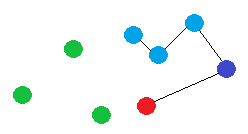
\includegraphics[width=0.65\textwidth]{./Imagenes/vecino4.png}
		\caption{Quinto vértice}
	\end{figure}
	\end{exampleblock}
\end{frame}


\begin{frame}
	\begin{exampleblock}{Paso 5}
	\begin{figure}[htbH]
		\centering
		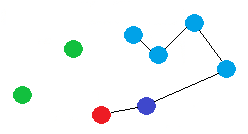
\includegraphics[width=0.65\textwidth]{./Imagenes/vecino5.png}
		\caption{Sexto vértice}
	\end{figure}
	\end{exampleblock}
\end{frame}

\begin{frame}
	\begin{exampleblock}{Paso 6}
	\begin{figure}[htbH]
		\centering
		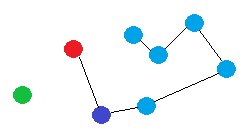
\includegraphics[width=0.65\textwidth]{./Imagenes/vecino6.png}
		\caption{Séptimo vértice}
	\end{figure}
	\end{exampleblock}
\end{frame}


\begin{frame}
	\begin{exampleblock}{Paso 7}
	\begin{figure}[htbH]
		\centering
		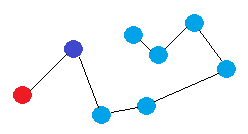
\includegraphics[width=0.65\textwidth]{./Imagenes/vecino7.png}
		\caption{Octavo y último vértice}
	\end{figure}
	\end{exampleblock}
\end{frame}

\begin{frame}
	\begin{exampleblock}{Paso 8}
	\begin{figure}[htbH]
		\centering
		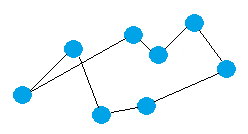
\includegraphics[width=0.65\textwidth]{./Imagenes/vecino8.png}
		\caption{Recorrido vecino más cercano}
	\end{figure}
	\end{exampleblock}
\end{frame}


\subsubsection{Eficiencia}
\begin{frame}
	\begin{block}{Calculo de la eficiencia}
	Cada ciudad la denotamos como $x_i = (i_a,i_b), i \in \{ 0,1,...n-1 \} $
	
	Y definimos la distancia entre dos ciudades como
	$dist(x_i, x_j) = \sqrt{ (i_a-j_a)^2 + (i_b-j_b)^2 }$
	\end{block}
	
	\begin{block}{ }
	En cada paso el cálculo del mínimo tiene que comprobar que la nueva ciudad no forme
	ciclo (pasar\'iamos dos veces por la misma ciudad)
	
	Definimos 
	$\phi (x_i) = \{ j \in A : min\{ dist(x_i,x_j)\} \ y \ no \ forme \ ciclos \}$
	\end{block}
\end{frame}

\begin{frame}
	\begin{block}{ }
	Comprobar si una ciudad forma ciclos es lineal, por lo que tenemos que $\phi (x_i)$
	es cuadrático.
	Debemos pasar por las $n$ ciudades, por lo que su eficiencia es:
	\[\sum_{k=0}^{n-1}\phi (x_k) \implies O(n) = n^3\]
	\end{block}
\end{frame}


\subsubsection{Ejemplos}
\begin{frame}
	\begin{exampleblock}{Puntos}
	\begin{figure}[htbH]
		\centering
		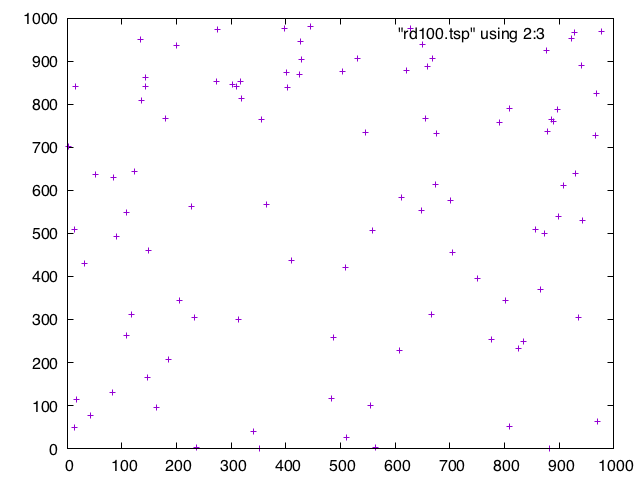
\includegraphics[width=0.65\textwidth]{../Viajante/Imagenes/rd100.png}
		\caption{Quinto vértice}
	\end{figure}
	\end{exampleblock}
\end{frame}

\begin{frame}
	\begin{exampleblock}{ Recorrido óptimo}
	\begin{figure}[htbH]
		\centering
		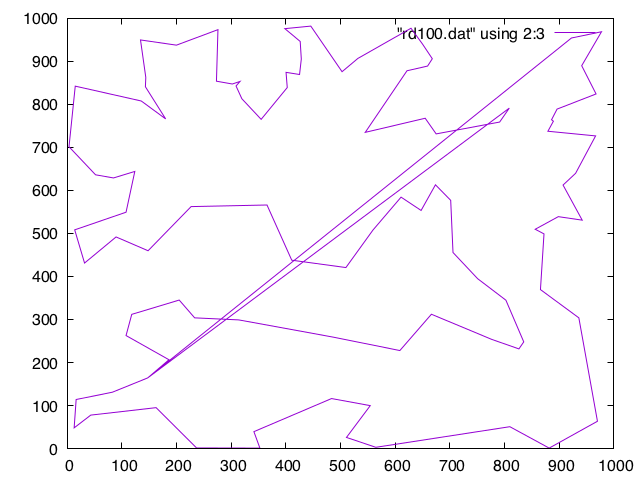
\includegraphics[width=0.65\textwidth]{../Viajante/Imagenes/rd100_opt.png}
		\caption{Quinto vértice}
	\end{figure}
	\end{exampleblock}
\end{frame}




%%%%%%%%%%%%%%%%%%%%%%%%%%%%%%%%%%%%%%%%%%%%%% Inserción
\subsection{Inserción de vértices}
\subsubsection{Explicación}
\begin{frame}
	\begin{block}{ }
El recorrido parcial inicial lo determinan los 3 puntos que estén más al Este, Oeste y Norte respectivamente. Los 3 no deben ser los mismos, algo que nunca pasa, pues 2 de ellos pueden ser iguales (un punto puede ser a la vez el punto más al Norte y al Este), pero 3 a la vez no.
	\end{block}

	\begin{block}{ }
	El nodo siguiente a insertar en el recorrido parcial será un nodo arbitrario, de lo 
	que nos encargaremos para hacer funcionar el greedy es de insertarlo entre los dos 
	vértices que más convengan, minimizar la distancia del circuito resultante.

	Pasaremos por todos los vértices que nos quedan cada vez, y sobre cada uno calculamos 
	la posición que más nos convenga dentro del circuito, y luego escogemos el vértice que 
	nos da mejor resultado.
	\end{block}
\end{frame}

\subsubsection{Eficiencia}
\begin{frame}
	\begin{block}
	Tenemos que recorrer $n$ vértices, y sobre cada uno de ellos aplicaremos una función 		
	$\phi(x)$ para cada vértice.

	\[ \sum_{i=1}^{n} \phi(x_i)\]
	\end{block}
	\begin{block}
	Dicha función $\phi(x)$ llama a "buscar punto" que es lineal, cada vez que buscas un 
	punto llama $n$ veces a "buscar posicion", que a su vez llama $n$ veces a calcular 
	longitud.

	Por tanto $\phi(x)$ es cúbica, y la eficiencia que nos queda para el algoritmo de 
	inserción es
	\[ O(n) = n^4 \]
	\end{block}
\end{frame}

\subsubsection{Ejemplos}

\begin{frame}
	\begin{exampleblock}{Puntos}
	\begin{figure}[htbH]
		\centering
		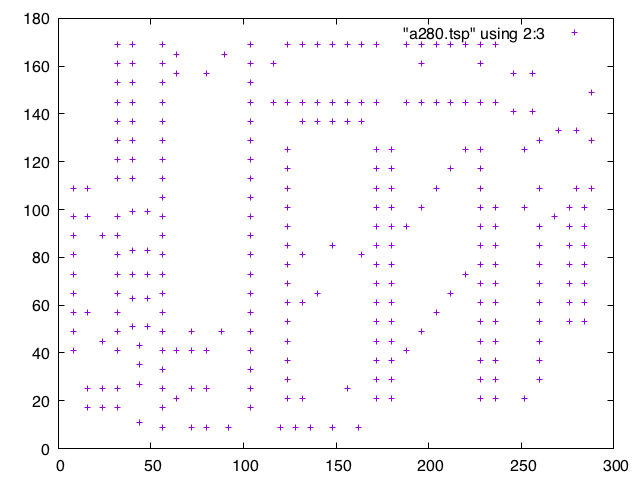
\includegraphics[width=0.65\textwidth]{../Viajante/Imagenes/a280.png}
		\caption{Quinto vértice}
	\end{figure}
	\end{exampleblock}
\end{frame}

\begin{frame}
	\begin{exampleblock}{Recorrido óptimo}
	\begin{figure}[htbH]
		\centering
		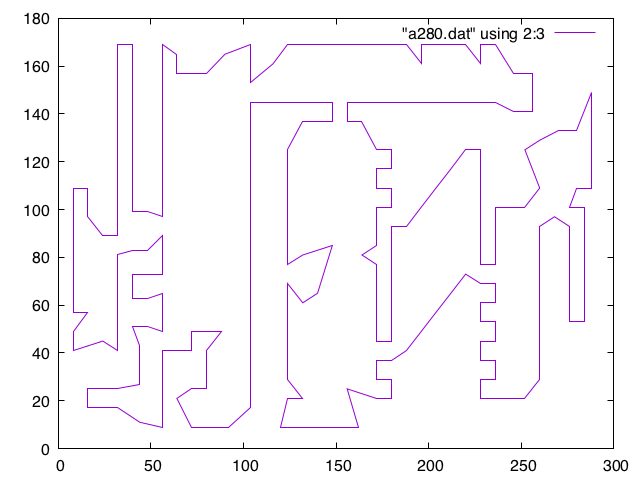
\includegraphics[width=0.65\textwidth]{../Viajante/Imagenes/a280_opt.png}
		\caption{Quinto vértice}
	\end{figure}
	\end{exampleblock}
\end{frame}

















%%%%%%%%%%%%%%%%%%%%%%%%%%%%%%%%%%%%%%%%%%%%%% Arista más cercana
\subsection{Inserción de aristas}
\subsubsection{Explicación}

\begin{frame}
	\begin{block}{  }
	Estrategia que consiste en ir seleccionando las aristas de menor longitud.
	
	Primero crearemos una clase Arista donde guardaremos los índices de los puntos dentro 
	del grafo (índices de ambos vértices de la arista) y la distancia entre ellos, sacada 
	de la matriz de adyacencia del grafo.
	
	Posteriormente ordenaremos todas las aristas en un vector, e iremos seleccionando 
	hasta pasar por todos los vértices una única vez, comprobando en cada paso que no 
	forme nuevos ciclos.
	\end{block}
	
	\begin{block}
	Definimos una relación de orden entre aristas de la siguiente forma:

	Una arista es \textit{menor que} otra si la distancia entre sus puntos es menor que la 
	distancia entre los puntos de la segunda arista.
	\end{block}
\end{frame}

\subsubsection{Comprobación de ciclo constante}
\begin{frame}
	\begin{block}{ }
	Hemos usado un vector de listas de aristas $vector < list <Edges> >$ .

	Cada lista definirá un camino inconexo con el resto de listas del vector, de forma que 
	su primer elemento y último sean los extremos.
	Al final del algoritmo nos quedará una única lista ordenada con la solución.
	\end{block}
		
	\begin{alertblock}{ }
	Para saber si una arista forma ciclo o no asignaremos un estado a cada vértice.
	\end{alertblock}
	
\end{frame}

\begin{frame}
	\begin{block}{ }
	Inicialmente los vértices tienen estado -1, significa que no han sido usados aún.
	Si se inserta una nueva arista, su primer vértice (inicio del camino) pasará al estado
	[1+10*posicion], siendo \textit{posicion} el lugar que ocupa dentro del vector de
	listas 
	
	El segundo vértice (último elemento) tendrá el estado [2+10*posicion]

	De esta forma si (estado1/10 == estado2/10) sabemos que los vértices están en el mismo 
	camino.
	\end{block}
	
	\begin{block}{ }
	Si hubiese vértices entre el principio y el final (cuando tenemos más de una arista) 
	los vértices intermedios tendrían estado [3+10*posicion]
	\end{block}
\end{frame}


\subsubsection{Casos posibles}
\begin{frame}
	\begin{block}
	Denotando como \textit{one} y \textit{two} los códigos de los vértices de la arista 
	que queremos insertar.
	\end{block}
\end{frame}
	
\begin{frame}
	\begin{block}{Caso 1}
	Ninguno está. En este caso se añadiría una nueva lista
	con una sola arista que nos indicaría que se ha creado un nuevo camino.
	\end{block}
	
	\begin{exampleblock}{Código}
	\hspace{1cm}((one == -1) \& \& (two == -1))
	\end{exampleblock}
\end{frame}	
	
\begin{frame}
	\begin{block}{Caso 2}
	Está uno y el otro está libre.
	\end{block}
	
	\begin{exampleblock}{Código} 
	\hspace{1cm}((one\%10 == 1) \& \& (two == -1) || (one\%10 == 2) \& \& (two == -1)    
	
	\hspace{1cm}(two\%10 == 1) \& \& (one == -1) || (two\%10 == 2) \& \& (one == -1) )
	\end{exampleblock}
\end{frame}

\begin{frame}
	\begin{block}{Caso 3}
	La arista une caminos, están los dos vértices, pero en caminos diferentes.
	Meteremos los elementos de la segunda lista de aristas en la primera
	\end{block}
	
	\begin{exampleblock}{Código}            
	\hspace{1cm}( ((one\%10 == 1) \& \& (two\%10 == 1) \& \& (one/10 != two/10)) ||
	               
	\hspace{1cm}((one\%10 == 2) \&\& (two\%10 == 2) \& \& (one/10 != two/10)) ||

	\hspace{1cm}((one\%10 == 1) \&\& (two\%10 == 2) \&\& (one/10 != two/10)) ||

	\hspace{1cm}((one\%10 == 2) \&\& (two\%10 == 1) \&\& (one/10 != two/10)) )
	\end{exampleblock}
\end{frame}
           
%%%%%%%%%%%%%%%%%%%%%%%%%%%%%%%%%%%%%%%%%5

\subsubsection{Eficiencia}
\begin{frame}
	\begin{block}{ }
	Siendo $n$ el número de puntos del grafo, para ordenar las $n^2$ aristas usaremos el 	
	Heapsort, por tanto obtenemos una eficiencia de $n^2log(n^2) \implies n^2log(n)$.
	\end{block}
	
	\begin{block}{ }
	En el peor caso recorreremos las $n^2$ aristas hasta encontrar las $n$ aristas  	
	deseadas.

	Como el algoritmo para ver si una arista forma ciclo es constante, si forma ciclo 
	pasará a la siguiente iteración, si no forma añadirá dicha arista.
	\end{block}
\end{frame}

\subsubsection{Explicación gráfica}

\begin{frame}
	\begin{exampleblock}{ }
	\begin{figure}[htbH] 
		\centering
		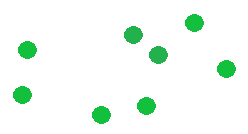
\includegraphics[width=0.5\textwidth]{./Imagenes/arista1.png}
		\caption{Eligiendo punto de inicio en azul} 
	\end{figure}
	\end{exampleblock}
\end{frame}

\begin{frame}
	\begin{exampleblock}{ }
	\begin{figure}[htbH] 
		\centering
		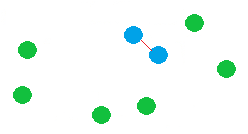
\includegraphics[width=0.5\textwidth]{./Imagenes/arista2.png}
		\caption{Tercer vértice} 
	\end{figure}
	\end{exampleblock}
\end{frame}

\begin{frame}
	\begin{exampleblock}{ }
	\begin{figure}[htbH] 
		\centering
		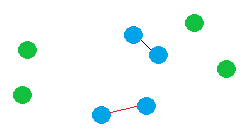
\includegraphics[width=0.5\textwidth]{./Imagenes/arista3.png}
		\caption{Cuarto vértice} 
	\end{figure}
	\end{exampleblock}
\end{frame}	

\begin{frame}
	\begin{exampleblock}{ }
	\begin{figure}[htbH] 
		\centering
		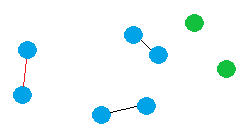
\includegraphics[width=0.5\textwidth]{./Imagenes/arista4.png}
		\caption{Quinto vértice} 
	\end{figure}
	\end{exampleblock}
\end{frame}

\begin{frame}
	\begin{exampleblock}{ }
	\begin{figure}[htbH] 
		\centering
		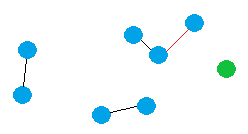
\includegraphics[width=0.5\textwidth]{./Imagenes/arista5.png}
		\caption{Sexto vértice} 
	\end{figure}
	\end{exampleblock}
\end{frame}

\begin{frame}
	\begin{exampleblock}{ }
	\begin{figure}[htbH] 
		\centering
		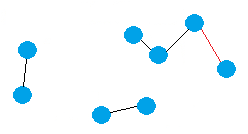
\includegraphics[width=0.5\textwidth]{./Imagenes/arista6.png}
		\caption{Séptimo vértice} 
	\end{figure}
	\end{exampleblock}
\end{frame}

\begin{frame}
	\begin{alertblock}{Ojo} 
	Debemos tener en cuenta que solamente podemos unir aristas que estén en dos caminos 
	diferentes si sus puntos son extremos de caminos ya existentes. De esta forma aunque 
	un vértice sea un extremo de un camino, si su otro extremo está en mitad de otro 
	camino no nos vale, ya que llegaría un punto en el que pasaríamos dos veces por el 
	mismo punto.
	\end{alertblock}
\end{frame}

\begin{frame}
	\begin{exampleblock}{ }
	\begin{figure}[htbH] 
		\centering
		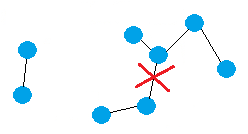
\includegraphics[width=0.5\textwidth]{./Imagenes/arista6fail.png}
		\caption{Octavo y último vértice} 
	\end{figure}
	\end{exampleblock}
\end{frame}		
	

\begin{frame}
	\begin{exampleblock}{ } 
	\begin{figure}[htbH] 
		\centering
		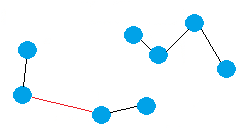
\includegraphics[width=0.5\textwidth]{./Imagenes/arista7.png}
		\caption{Octavo y último vértice} 
	\end{figure}
	\end{exampleblock}
\end{frame}


\begin{frame}
	\begin{exampleblock}{ } 
	\begin{figure}[htbH] 
		\centering
		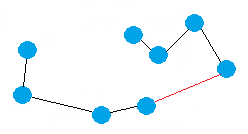
\includegraphics[width=0.5\textwidth]{./Imagenes/arista8.png}
		\caption{Octavo y último vértice} 
	\end{figure}
	\end{exampleblock}
\end{frame}

\begin{frame}
	\begin{exampleblock}{ }
	\begin{figure}[htbH] 
		\centering
		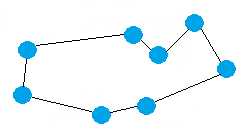
\includegraphics[width=0.5\textwidth]{./Imagenes/arista9.png}
		\caption{Recorrido vecino más cercano} 
	\end{figure}
	\end{exampleblock}
\end{frame}



\subsubsection{Ejemplos}
\begin{frame}
	\begin{exampleblock}{Puntos}
	\begin{figure}[htbH]
		\centering
		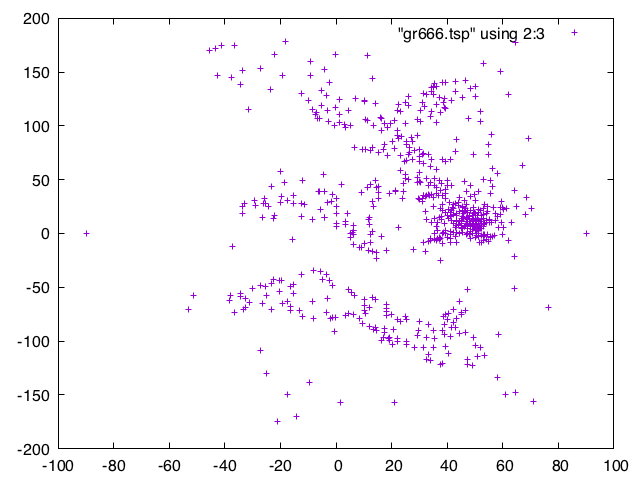
\includegraphics[width=0.65\textwidth]{../Viajante/Imagenes/gr666.png}
		\caption{Quinto vértice}
	\end{figure}
	\end{exampleblock}
\end{frame}
	
\begin{frame}
	\begin{exampleblock}{Recorrido óptimo}
	\begin{figure}[htbH]
		\centering
		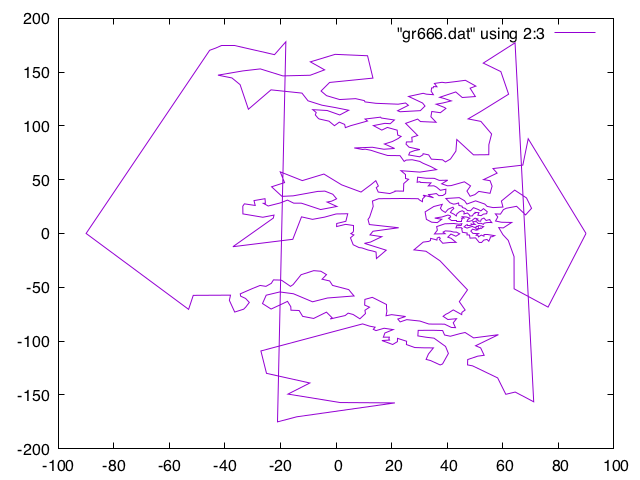
\includegraphics[width=0.65\textwidth]{../Viajante/Imagenes/gr666_opt.png}
		\caption{Quinto vértice}
	\end{figure}
	\end{exampleblock}
\end{frame}